\chapter{Zebrane doświadczenia}
\label{Chapter8}

\section{Problemy i ich rozwiązania}
\subsection{Maciej Trojan}
\subsubsection{Inicjalizacja bazy danych}
Moduł iQuest do działania wymaga rozszerzenie istniejącej bazy danych platformy \emph{Moodle} o dodatkowe tabele, przechowujące niezbędne dane wykorzystywane do spełnienia założonej funkcjonalności.

Do zaimportowania bazy danych przygotowanej przez architekta wykorzystano narzędzie, wbudowane w platformę \emph{Moodle}, \emph{XMLDB}, które gwarantuje bezobsługową instalację modułu w przyszłości. Jak się później okazało narzędzie to posiada błąd, który uniemożliwia zaimportowania kluczy obcych. Wymagało to od programistów ręcznego utworzenia wszystkich kluczy obcych, przewidzianych przez architekta.

\subsubsection{Instalacja modułu}
Postanowiono, że wraz z instalacją modułu powinień automatycznie tworzyć się odpowiedni \emph{kurs} związany jedynie z modułem \emph{iQuest}. Zmniejsza to potrzebny czas na przygotowanie platformy do użytku, oraz zapobiega pomyłkom związanych z ręcznym tworzeniem i konfiguracji \emph{kursu}. 

Niestety okazało się, że podejście to uniemożliwia instalację modułu jednocześnie z całą platformą \emph{Moodle}, ponieważ dodatkowe moduły instalowane są przed mechanizmami pozwalającymi na tworzenie \emph{kursu}. Doinstalowanie modułu do zainstalowanej platformy nie powoduje żadnych komplikacji.

\subsection{Krzysztof Urbaniak}
\subsubsection{Wprowadzenie}
Na początku tego rozdziału należy przypomnieć, główne pojęcia związane z korzystaniem z platformy \emph{Moodle}.

Po zalogowaniu do systemu użytkownik musi wybrać \emph{kurs}. Kurs jest największą częścią \emph{Moodle} i przeważnie kojarzony jest z przedmiotem. Na kurs składa się kilka lub kilkanaście \emph{sekcji}. Sekcja odpowiada najczęściej konkretnym zajęciom, jest związana z jakimś wydarzeniem lub tygodniem. Najmniejszą jednostką w \emph{Moodle} jest \emph{aktywność}. Aktywność to podstawowy typ modułów rozszerzających funkcjonalność \emph{Moodle}. Aktywnościami są np. \emph{Forum}, \emph{Głosowanie}, \emph{Czat}. Istnieje również inny typ modułów: \emph{zasoby}. Są to m.in. własne strony internetowe, pliki, adresy \emph{URL}. Na potrzeby projektu została wyróżniona grupa \emph{materiały}. Zalicza się do niej wszystkie moduły inne niż \emph{iQuest}, czyli inne niż badania. Moduły grupowane są w sekcje.

\emph{Formater} kursu decyduje o ułożeniu i wyświetlaniu elementów na stronie.

Różnica pomiędzy tym, czy użytkownik znajduje się lub nie, w module lub w kursie, to \emph{kontekst}.

Jako, że rozdział ten tyczy się grafiki, warto wspomnieć, że elementy na stronie ułożone są w następujący sposób:
\begin{description}
\item Na ekranie wyświetlana jest lista sekcji.
\item Wewnątrz każdej sekcji znajduje się lista badań. Pod nią drukowana jest lista materiałów.
\end{description}

\subsubsection{Formularze}
Projektując graficzny interfejs użytkownika, prędzej, czy później pojawia się potrzeba wyboru narzędzia do projektowania formularzy. Rozważano kilka możliwości. Po pierwsze, użycie po prostu czystego języka \emph{HTML}. Drugą opcją było użycie wbudowanych w \emph{Moodle} \emph{API} -- \emph{Form API} lub \emph{Output API}. Jako trzecią możliwość rozważano użycie zewnętrznych \emph{API} -- nie związanych z \emph{Moodle}.

Odrzucono pomysł pierwszy oraz trzeci. Pomysł pierwszy wydał się zbyt pracochłonny. Z uwagi na dość mocno ograniczony czas, niemądrze byłoby programować coś od początku samemu, skoro ktoś inny już coś podobnego napisał. Nawet kosztem tego, że interfejs nie wyglądał dokładnie tak, jak go zaprojektowano. Ważne, aby był kompletny. Wariant trzeci był nie zgodny z założeniem mówiącym o korzystaniu z interfejsów \emph{Moodle} tam, gdzie to możliwe. Nie chciano, żeby użytkownik poczuł, że programowana wtyczka nie jest częścią systemu \emph{Moodle}. Co więcej, interfejs odbiegałby od wyglądu \emph{Moodle} i mógłby zostać oceniony jako nieintuicyjny. Zdecydowano się korzystać z \emph{Output API}.

\emph{Output API} to zestaw funkcji, wprowadzonych od wersji \emph{Moodle} $2.0$. Umożliwiają one wstawianie na stronę standardowych elementów formularza, takich jak: etykiety, przyciski, linki, tabele etc. Niestety, z nieznanych powodów, to wspaniale wyposażone, z pełną dokumentacją i w pełni przydatne \emph{API} zostało usunięte z \emph{Moodle} już w wersji $2.2$. Co ciekawe niektórych elementów można nadal używać, lecz nie znaleziono dokumentu, który mówiłby o tym jakie dokładnie części tego \emph{API} można używać, a które zostały wycofane.

Następcą \emph{Output API} został \emph{Form API}. Ku rozczarowaniu zespołu \emph{Form API} ma nieco uboższą dokumentację. Zdarza się, że w funkcji są omówione np. tylko trzy pierwsze argumenty, natomiast reszta jest pominięta, tak jakby nie istniała. \emph{Form API} różni się też od poprzednich \emph{API} tym, że jest oparte na modelu obiektowym. Posiada także mechanizm pozwalający na weryfikację danych, wprowadzanych przez użytkownika. Mechanizm ten napisany jest z użyciem języka \emph{JavaScript}, oznacza to, że walidacja przeprowadzana jest po stronie klienta, a dopiero poprawne dane przesyłane są do serwera.

Podsumowując, mimo niekompletnej dokumentacji, jako narzędzie implementacji formularzy, zostało wybrane \emph{Form API}. Posiada ono szereg przydatnych funkcji, pozwalających na definiowanie standardowych elementów każdego formularza. Nie bez znaczenia są też funkcje pozwalające na walidację wprowadzanych danych. Oczywiście nie wszystkie potrzebne elementy udało się napisać używając jedynie \emph{API}. Korzystano wtedy z czystego języka \emph{HTML}. 

\subsubsection{Role}
Jedną z cech projektu, jest podział użytkowników na ankieterów i respondentów. W systemie \emph{Moodle} istnieje mechanizm do zarządzania rolami, który wydawał się adekwatny do użycia w tym przypadku. Rola jest to zbiór \emph{możliwości}. Możliwość można rozumieć jako prawo do wykonania, określonego przez programistę, fragmentu kodu.

\subsubsection{Formater kursu}
Jednym z problemów jakie napotkano, była konieczność wyświetlania respondentom i ankieterom tylko określonych modułów. Ankieterzy powinni zobaczyć tylko te badania, które utworzyli oraz inne aktywności, zasoby. Respondenci powinni zobaczyć tylko te badania, w których mogą wypełnić ankietę, a także materiały, które mają prawo wyświetlać.

Do rozwiązania problemu zdecydowano się użyć formatera kursu. Narzędzie to, jako integralna część \emph{Moodle}, było najlepszym rozwiązaniem z możliwych. Niestety wkrótce okazało się, że brak dokumentacji, a także dyskusji na temat tego narzędzia w internecie utrudnia wykonanie zadania. Całą pracę wejścia, polegającą na poznaniu narzędzia, wykonano studiując kod źródłowy domyślnych formaterów \emph{Moodle}.

Pierwszy plan zakładał wyświetlanie użytkownikowi dwóch sekcji. Jedną z odpowiednimi badaniami, drugą z materiałami. Należało także ograniczyć ankieterowi możliwość dodawania w pierwszej sekcji modułów innych niż iQuest, a w drugiej sekcji uniemożliwić dodanie tej aktywności. Niestety wyszło na jaw, że jest to nieosiągalne bez ingerowania w wewnętrzny kod platformy \emph{Moodle}. 

Zostało to spowodowane uaktualnieniami w \emph{Moodle}. Kod \emph{PHP} wyświetlania typów modułów, zostaje nadpisywany przez \emph{JavaScript}. W taki sposób, z poziomu funkcji \emph{PHP}, odpowiedzialnych za wyświetlanie listy modułów w danej sekcji, nie da się kontrolować, które moduły zostaną wyświetlane, a które nie. Mówiąc prościej, programista może jedynie wybrać, jakie moduły będą wyświetlane we wszystkich sekcjach w danym kursie, a nie może decydować o tym, co można dodać w każdej sekcji z osobna.

Rozwiązaniem było umieszczenie listy badań oraz listy materiałów w jednej sekcji. Można w niej dodać jakikolwiek moduł. Dopiero przy wyświetlaniu moduły dzielone są na dwie listy: listę badań i listę materiałów. Dzięki temu cel został osiągnięty -- użytkownik zobaczy tylko te moduły, które może wyświetlić. Co więcej, będą one odpowiednio posegregowane, aby użytkownik szybko mógł znaleźć to, czym jest zainteresowany.

\subsubsection{Tworzenie badania}
Kolejną trudnością w projekcie, było połączenie go z systemem \emph{Moodle}. Głównie sprowadzało się to do tego, aby tak wykorzystać interfejs graficzny oferowany przez \emph{Moodle}, żeby użytkownik nie miał poczucia zmiany systemu. Zarówno wygląd, jak i dodawanie różnych funkcji, powinny być zgodne ze standardem \emph{Moodle}. Dzięki takiemu podejściu, osoba, korzystająca wcześniej z \emph{Moodle}, a pragnąca używać wtyczki \emph{iQuest}, nie musiała zmieniać swoich przyzwyczajeń. Co więcej, w projekcie duży nacisk został postawiony na nie zniechęcanie respondentów do wypełnienia ankiety, co było dodatkową motywacją do zaprojektowania przyjaznego użytkownikom interfejsu.

Wstępna wersja interfejsu, zaprojektowana przez architekta, wyglądała następująco. Najpierw ankieter wyrażał chęć utworzenia nowego badania, klikając odpowiedni przycisk. Następnie mógł dodać do badania ankietę z katalogu, ewentualnie utworzyć nową. Na kolejnej stronie ankieter definiował szczegóły badania, takie jak: nazwa, grupa docelowa, czas rozpoczęcia i zakończenia etc. Nie było możliwe, aby zaimplementować to w powyższy sposób.

Problem stwarzało dodawanie ankiety wewnątrz tworzenia badania. Gdy tworzenie badania zaczyna się od zdefiniowania ankiety, to nie można od razu dodać jej do odpowiedniego badania, ponieważ to badanie jeszcze nie istnieje. W takim wypadku należałoby przechowywać gdzieś informację, że po utworzeniu badania ma dodać się do niego ankieta. Na przykład można w tym celu użyć dodatkowy parametr w adresie \emph{URL}. Dodatkowo, w \emph{Moodle}, przy kreowaniu nowego modułu, użytkownikowi wyświetlany jest domyślny formularz, w którym podaje się parametry potrzebne do zbudowania instancji modułu. Przyjmując, że badanie jest kojarzone z modułem, nie ma możliwości, aby przed zakończeniem tworzenia badania wstawić dodatkowy formularz.

Rozwiązaniem jest prosta zamiana kolejności tworzenia badania oraz ankiety. Najpierw użytkownik tworzy badanie, czyli moduł. Dopiero wówczas ma możliwość sporządzenia ankiety. Podejście to ma kilka zalet: jest to zgodne z procedurą \emph{Moodle}, a co za tym idzie, bardziej intuicyjne dla użytkownika obeznanego z \emph{Moodle} oraz pozwala na łatwe dodanie ankiety do badania. Ponadto ankieter może zrezygnować z komponowania ankiety przy kreowaniu badania. Nie sposób nie zgodzić się z tezą, że jest to jedyny słuszny sposób dodawania nowego modułu \emph{iQuest}.

\subsubsection{Tworzenie ankiety}
Przy tworzeniu ankiety powstał dość specyficzny problem implementacyjny. Wynikał on z faktu, że ankietę definiować można zarówno z poziomu kursu, jak i z poziomu badania. Powstało pytanie: Jak przetwarzać dane pochodzące z różnych kontekstów? 

Standardowo, we wtyczkach Moodle, elementy odpowiedzialne za wyświetlanie informacji na ekranie znajdują się w pliku \emph{view.php}. Pojawił się pomysł, aby rozszerzyć strukturę o dwa dodatkowe pliki: \emph{mod.php} oraz \emph{course.php}. Do pliku \emph{mod.php} trafiały dane z kontekstu modułu. Drugi plik zajmował się przetwarzaniem danych z kontekstu kursu. Taki podział gwarantował większy porządek w kodzie źródłowym. Porządek był ważny, ponieważ w \emph{Moodle} nie jest zgodny z wzorcem Model-View-Controller. W związku z tym ważne jest aby efektywnie zarządzać kodem źródłowym, żeby mała jego zmiana nie wymagała zmiany wielu elementów.

Niestety wprowadzone zmiany okazały się niewystarczające. Występowało niepotrzebne powielanie kodu. Wydzielono jeszcze jeden plik, w którym przetwarzano dane otrzymane z formularzy, zapisywano je do bazy danych. Później zwracano sterowanie do plików \emph{mod.php} albo \emph{course.php} w zależności od kontekstu.

Dzięki utworzeniu trzech dodatkowych plików, kod źródłowy stał się bardziej przejrzysty. Wartość takiego rozwiązania można zauważyć dopiero, gdy zachodzi konieczność znalezienia błędu lub wprowadzenia zmian. Przy dobrym zarządzaniu kodem mała zmiana wymaga małych zmian.

\subsubsection{Inwencja programistów}

W trakcie rozwoju oprogramowania pojawiło się kilka małych niejasności, które programiści musieli rozwiązać sami. Kilka razy wykazali również inicjatywę i zaproponowali rozwiązania, które stały się ostatecznie częścią projektu.

Pierwszą ideą było zagospodarowanie przestrzeni w widoku badania. Po utworzeniu badania i dodania do niego ankiety, ankieterowi ukazuje się widok badania. Architekt nie zaproponował jak ma on wyglądać. Dał tylko pewne wskazówki. Zaznaczył, że z tego widoku, ankieter ma mieć możliwość usunięcia ankiety z badania oraz edytowania jej. I tu pojawił się problem. Żeby spełnić wymagania, na stronie wystarczyło pokazać odnośniki: ,,edytuj'' i ,,usuń z badania''. Praktycznie cała stron pozostawała pusta. Sytuacja taka jest niedopuszczalna, bo na pewno istniały jakieś przydatne informacje, które można było w tym miejscu wyświetlić. Wykoncypowano, że najbardziej naturalnie będzie pokazać w tym miejscu statystyki dla badania.

W pierwszej wersji zaimplementowano tylko proste statystyki. Można się z nich dowiedzieć: ile czasu zostało do zakończenia badania, ile osób liczy grupa docelowa oraz ile osób już odpowiedziało i poznać wartość procentową. Następnie dodano kolejną tabelkę ze statystykami. Wyświetla się gdy choć jedna osoba odpowie na któreś pytanie. Możemy w niej zobaczyć jak kształtowały się odpowiedzi, w pytaniach zamkniętych, na które odpowiedziano. Nie zdecydowano się wyświetlać odpowiedzi na pytania otwarte ze względu na ich różnorodność, a więc ilość miejsca, które zajmowały. Ideą tabelki było pokazanie skróconych informacji o badaniu. Cały, dokładny, rozbudowany raport można wygenerować z użyciem systemu \emph{Jasper Report}.

Pozyskanie i podliczenie odpowiedzi na dane pytanie wiązało się z wymyśleniem algorytmu. Teoretycznie najprostszym rozwiązaniem byłoby, dla każdej dozwolonej odpowiedzi na pytanie zamknięte, sprawdzenie liczności krotek w tabeli \emph{answers}. To rozwiązanie jest jednak nieoptymalne, bo wiąże się z wielokrotnym odwoływaniem się do bazy danych. Lepiej pozwolić bazie danych samej zoptymalizować odwołania do tablic. Tak postąpiono w tym przypadku. Przy użyciu wyrażenia ,,GROUP BY'' opracowano zapytanie, które od razu zwracało liczbę odpowiedzi respondentów na możliwą odpowiedź. Takie podejście gwarantuje szybsze wykonanie algorytmu.

Kolejnym pomysłem programistów było dodanie kilku przycisków. Zarówno w katalogu jak i widoku badania umieszczono przycisk ,,pokaż''. Służy on do wyświetlenia ankiety tak samo jak widzi ją respondent. Ankieter może zobaczyć, układ pytań, łatwiej mu zdecydować o dodaniu kolejnej strony. Pojawił się także przycisk pozwalający na dodanie nowej ankiety, będąc w widoku katalogu. Znajduję się on zarówno na dole jak i na górze tabelki, aby nie było konieczności przewijania ekranu.

W założeniach projektu ustalono, że odpowiedź jest nieedytowalna. Dodano udoskonalenie, które polegało na tym, że respondent nie musi od razu wypełnić całej ankiet. Może to robić stopniowo. Za każdym razem jednak zostaną mu wyświetlone tylko te pytania, na które jeszcze nie odpowiedział. Pozwala to także uniknąć sytuacji, w której respondent przeoczy jakieś pytania. Jeśli respondent nie wypełni całej ankiety, to badanie nie zniknie z widoku kursu. Dopiero po wypełnieniu całej ankiety badanie nie pokaże się w kursie.

\subsection{Łukasz Wieczorek}
\subsubsection{Mapowanie obiektowo-relacyjne}
Mapowanie obiektowo-relacyjne pozwala uprościć operacje na danych przechowywanych w bazie danych poprzez udostępnienie ich programiście w postaci obiektowej.\\
System \emph{iQuest} operuje na klasach takich jak: ankieta, badanie, grupa docelowa, członek grupy docelowej, uprawnienie dostępu, pytanie (i potomne), odpowiedź, zadanie, praca w tle, etc. Początkowo architekt stworzył diagram klas na którym każda klasa miała wyróżnione publiczne metody \emph{insert, update, delete}. Niestety takie rozwiązanie spowodowało powielenie dużej ilości kodu związanego z interakcją z bazą danych. W ramach refaktoryzacji podjąłem się zadania stworzenia klas, które wzorem nowoczesnych systemów \emph{ORM} uproszczą projektowanie nowych klas reprezentujących dane. Ze względu na silną integrację z mechanizmami \emph{Moodle} w grę nie wchodziły gotowe rozwiązania. Autorskie rozwiązanie korzysta z mechanizmów \emph{Moodle Data manipulation API} oraz mechanizmu refleksji języka PHP, by pozwolić programiście korzystającego z tego rozwiązania na proste pobieranie i manipulację obiektami przechowywanymi w bazie danych. Diagram UML przedstawia się następująco:
\begin{figure}[!th]
\centering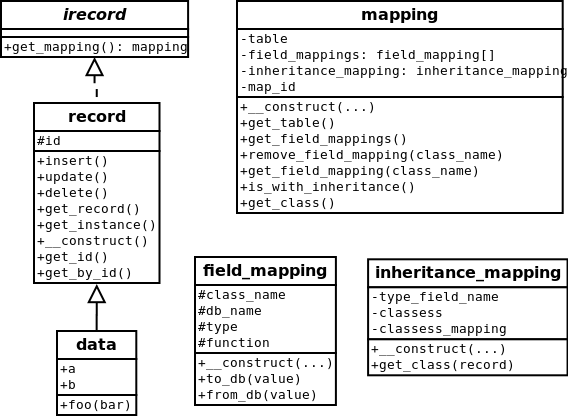
\includegraphics[width=15cm]{figures/lw/iquest-orm.png}
\caption{iQuest ORM}\label{rys:iquest-orm}
\end{figure}
Klasa danych dziedziczy po klasie \emph{record} oraz implementuje metodę \emph{get\_mapping} interfejsu \emph{irecord}, by uzyskać dostęp do metod komunikacji z bazą danych. Metoda \emph{get\_mapping} pozwala zdefiniować mapowanie danej klasy na odpowiednią relację w bazie danych. Należy przy tym podać mapowania dla atrybutów, tj. nazwy w klasie i bazie danych oraz typ, który zadecyduje o metodzie pobrania/zapisania danej (typem może być także klasa potomna klasy \emph{record}). W przypadku, gdy mamy do czynienia z dziedziczeniem wystarczy zdefiniować przy mapowaniu sposób obsługi dziedziczenia (m.in. jakie pole określa typ klasy). Najważniejszy kod znajduje się w metodzie \emph{get\_instance}, która pobiera konstruktor danej klasy, poprzez refleksję tworzy obiekt z wyłuskanymi z bazy danych parametrami wymaganymi przy jego tworzeniu oraz ustawia resztę pól pobranych z bazy danych. Metody \emph{insert, update, delete} pobierają reprezentację obiektu oczekiwanego przez metody \emph{Data manipulation API} oraz wykonują żądane operacje.\\
Zastosowane rozwiązanie znacząco poprawiło czytelność kodu poprzez zastosowanie zasady DRY (\emph{Don't repeat yourself}). Projektowałem je, mając na uwadze rozwiązanie, z którym miałem wcześniej styczność, tj. implementację \emph{ActiveRecord} z \emph{Ruby on Rails}. W trakcie pracy nad projektem doceniłem stosowanie konwencji nazewniczych, których obecność znacząco upraszcza projektowanie klas mapujących dane.

%Tutaj znajduje się opis wszystkich Waszych doświadczeń związanych z projektem -- zarówno pozytywnych jak i negatywnych, dotyczących organizacji, środowiska czy samych już kwestii technicznych. To ma być zebranie Waszych wniosków, wraz z prawdopodobnymi nauczkami dla przyszłych roczników. 
%
%To dobre miejsce na zaaplikowanie zawartości Lessons Learned Log, jeśli tak prowadziliście, ale też miejsce na własne przemyślenia.